\section{Preuve rang 4}

\paragraph{}
Nous allons maintenant étudier les différents cas en rang 4. Nous pouvons avoir deux, trois ou quatre 4-transpositions. Étudions ces cas successivement.

\subsection{Deux 4-transpositions}

\paragraph{}
Remarquons qu'avec nos deux 4-transpositions, on 12 arêtes alors qu'il nous en faut 10. Nous en avons donc juste deux en trop.

\begin{theorem}
  Si un sggi de degré $4$ sur $A_{11}$ possède exactement deux 4-transposition, alors celles-ci sont sur les positions $\rho_1$ et $\rho_2$.
\end{theorem}

\begin{proof}
  Supposons qu'il existe une 4-transposition en $\rho_0$. Alors celle-ci doit commuter avec $\rho_2$ et $\rho_3$. Ces deux dernières involutions ont au moins deux arêtes chacunes.



  \paragraph{}
  Nous allons utiliser un raisonnement similaire à celui utilisé pour le rang 5. Néanmoins, une différence avec le rang 5 est que les deux involutions que nous ajoutons ($\rho_2$ et $\rho_3$) ne doivent pas commuter entre elles. Dès lors, il est possible, lors de la construction de $\rho_3$, de relier deux points fixés par $\rho_0$ mais pas fixés par $\rho_2$ sans que cela ne pose un problème. Les deux possibilités sont donc les suivantes.

  \begin{enumerate}
    \item Doubler une arête et relier deux points fixés par $\rho_0$.
    \item Former un carré alterné.
  \end{enumerate}

  \paragraph{}
  Le problème se pose quand on choisit ce que doit faire l'involution $\rho_3$. Elle ne peut pas former d'arête double avec $\rho_0$ car il est impossible de les relier après. De même, elle ne peut pas former de carré alterné avec $\rho_0$ car le problème serait le même. Il faut donc utiliser l'involution $\rho_2$ pour résoudre ce problème.

  \paragraph{}
  Pour relier l'arête double, la seule solution est de créer un carré qui contiendra cette arête mais alors ce carré possèderait une arête triple et donc on utiliserait trois arête disponibles alors que nous n'en possèdont que deux. Pour relier le carré alterné, nous pouvons coller un autre carré alterné à celui-ci. On obtient alors le graphe suivant:

  \begin{figure}[H]
    \begin{center}
      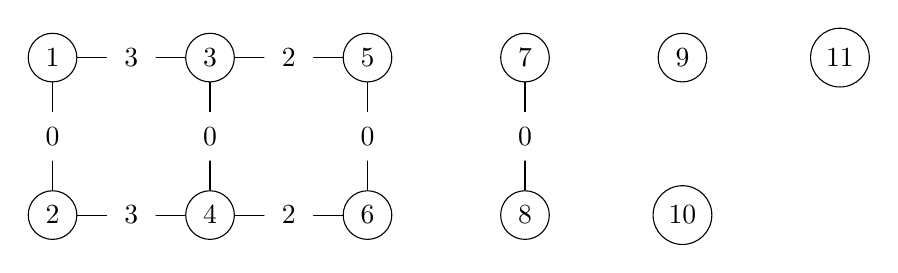
\begin{tikzpicture}

        \begin{scope}[every node/.style={circle,draw}]
          \node (1)  at (0,2)  {1};
          \node (2)  at (0,0)  {2};
          \node (3)  at (2,2)  {3};
          \node (4)  at (2,0)  {4};
          \node (5)  at (4,2)  {5};
          \node (6)  at (4,0)  {6};
          \node (7)  at (6,2)  {7};
          \node (8)  at (6,0)  {8};
          \node (9)  at (8,2)  {9};
          \node (10) at (8,0)  {10};
          \node (11) at (10,2) {11};
        \end{scope}

        \begin{scope}[every node/.style={fill=white,circle}]

          \begin{scope}[every edge/.style={draw}]
            \path (1)  edge node {$0$} (2);
            \path (3)  edge node {$0$} (4);
            \path (5)  edge node {$0$} (6);
            \path (7)  edge node {$0$} (8);
            \path (3)  edge node {$2$} (5);
            \path (4)  edge node {$2$} (6);
            \path (1)  edge node {$3$} (3);
            \path (2)  edge node {$3$} (4);
          \end{scope}
        \end{scope}

      \end{tikzpicture}
      \caption{}
    \end{center}
  \end{figure}

  \paragraph{}
  Maintenant la seule possibilité pour relier les carrés au reste est d'utiliser des arêtes de $\rho_1$. Nous allons donc devoir utiliser deux arêtes de $\rho_1$. Pour relier les points manquants nous avons alors un ou deux points que nous pouvons relier et celui-ci (ceux-ci) sont uniquement reliés par des arêtes de $\rho_1$. La seule possibilité est d'utiliser une arête de $\rho_2$ pour les relier. Donc $\rho_2$ est une 4-transposition. Étudions les deux cas un peu plus en détails.

  \paragraph{}
  Nous ne pouvons utiliser qu'une arête $\rho_2$. En effet dans le cas où nous n'avons qu'une arête $\rho_1$ où nous pouvons attacher qu'une seule arête $\rho_2$ car nous n'avons qu'un point disponible. Dans le cas où nous avons deux points connecté par $\rho_1$, ces deux point faisaient partie des trois points fixes du graphe ci-dessus. Il n'en reste plus qu'un, donc soit nous relions les deux points ensemble soit nous relier le dernier point fixe. Si nous relions les points ensemble, nous ne pouvons plus rien faire.

  \paragraph{}
  Maintenant, nous devons relier le dernier point que nous avons créé, qui est déjà relié par $\rho_2$. Mais nous ne pouvons plus utiliser $\rho_2$. Donc $\rho_2$ est une 3-transposition, ce qui est impossible.

\end{proof}

\begin{theorem}
  Tout sggi de rang 4 sur $A_{11}$, composé de deux 4-transpositions ne peut être un string C-group.
\end{theorem}

\begin{proof}
  Commençons par
\end{proof}

\subsection{Trois 4-transposisitions}

\begin{lemma}
  Pour un sggi de rang 4 sur $A_{11}$ composé de trois 4-transpositions, la 2-transposition restante sera en position $\rho_0$ (à la dualité près).
\end{lemma}

\begin{theorem}
  Tout sggi de rang 4 sur $A_{11}$, composé de trois 4-transpositions ne peut être un string C-group.
\end{theorem}

\begin{proof}
  Construisons donc les possibilités pour les 4-transpositions $\rho_1$ et $\rho_3$. Celles-ci doivent commuter. Mettons une première 4-transpositions, on a
  \begin{figure}[H]
    \begin{center}
      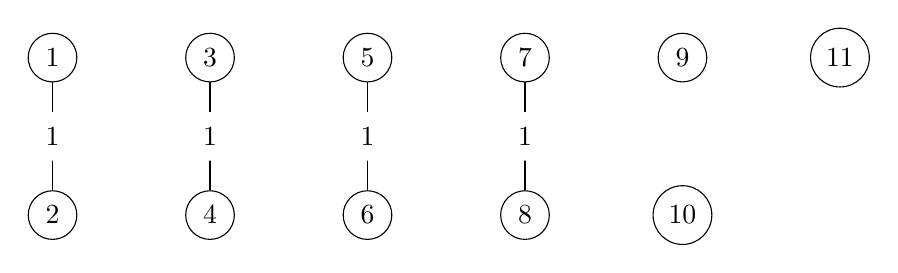
\begin{tikzpicture}

        \begin{scope}[every node/.style={circle,draw}]
          \node (1)  at (0,2)  {1};
          \node (2)  at (0,0)  {2};
          \node (3)  at (2,2)  {3};
          \node (4)  at (2,0)  {4};
          \node (5)  at (4,2)  {5};
          \node (6)  at (4,0)  {6};
          \node (7)  at (6,2)  {7};
          \node (8)  at (6,0)  {8};
          \node (9)  at (8,2)  {9};
          \node (10) at (8,0)  {10};
          \node (11) at (10,2) {11};
        \end{scope}

        \begin{scope}[every node/.style={fill=white,circle}]

          \begin{scope}[every edge/.style={draw}]
            \path (1)  edge node {$1$} (2);
            \path (3)  edge node {$1$} (4);
            \path (5)  edge node {$1$} (6);
            \path (7)  edge node {$1$} (8);
          \end{scope}
        \end{scope}

      \end{tikzpicture}
      \caption{}
    \end{center}
  \end{figure}

  \paragraph{}
  Nous voulons placer la 4-transposition $\rho_3$, en sachant qu'on doit pouvoir placer une 4-transposition $\rho_2$ après.

  \paragraph{}
  Si, lorsque nous plaçons l'involution $\rho_3$ de telle sorte qu'on ne relie que des points qui sont déjà permutés par $\rho_1$, on va toujours avoir deux points fixes et les 8 autres points seront permutés par les deux involutions. Dans une telle situation, il est impossible d'avoir un sggi. En effet, on a déjà utilisé les arêtes libres que nous avons et donc toutes les nouvelles arêtes doivent connecter des composantes distinctes. Mais il est impossible de relier les trois points fixes avec les involutions $\rho_0$ et $\rho_2$. En effet celles-ci doivent commuter mais on ne peut plus former de structure telle que cela soit possible.

  \paragraph{}
  Donc l'involution $\rho_3$ permutent deux points jusque là fixes. Pour conserver la parité, nous devons forcément doubler une arête de $\rho_1$. On a alors le graphe suivant

  \begin{figure}[H]
    \begin{center}
      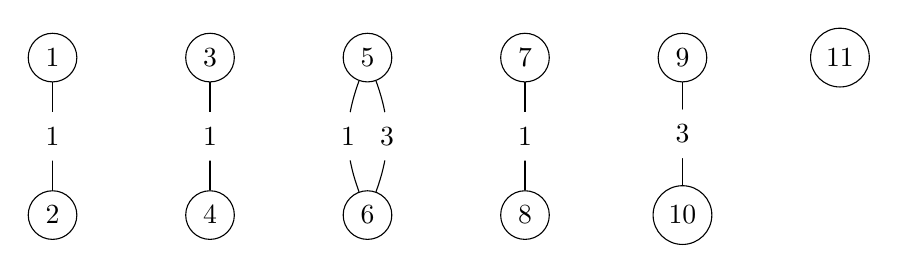
\begin{tikzpicture}

        \begin{scope}[every node/.style={circle,draw}]
          \node (1)  at (0,2)  {1};
          \node (2)  at (0,0)  {2};
          \node (3)  at (2,2)  {3};
          \node (4)  at (2,0)  {4};
          \node (5)  at (4,2)  {5};
          \node (6)  at (4,0)  {6};
          \node (7)  at (6,2)  {7};
          \node (8)  at (6,0)  {8};
          \node (9)  at (8,2)  {9};
          \node (10) at (8,0)  {10};
          \node (11) at (10,2) {11};
        \end{scope}

        \begin{scope}[every node/.style={fill=white,circle}]

          \begin{scope}[every edge/.style={draw}]
            \path (1)  edge node {$1$} (2);
            \path (3)  edge node {$1$} (4);
            \path (5)  edge[bend right=20] node {$1$} (6);
            \path (7)  edge node {$1$} (8);
            \path (5)  edge[bend left=20] node {$3$} (6);
            \path (9)  edge node {$3$} (10);
          \end{scope}
        \end{scope}

      \end{tikzpicture}
      \caption{}
    \end{center}
  \end{figure}

  \paragraph{}
  Concernant les deux arêtes restantes pour $\rho_3$, nous pouvons soit les utiliser pour doubler deux arêtes, soit pour former un carré alterné. Le cas des deux arêtes est impossible car il ne nous resterait qu'un seule arête libre. Donc il faudrait forcément doubler une arête $\rho_2$ qui doit être contenue entre des arêtes $\rho_1$ mais ça n'existe pas. Donc les deux dernières arêtes forment un carré alterné.

  \begin{figure}[H]
    \begin{center}
      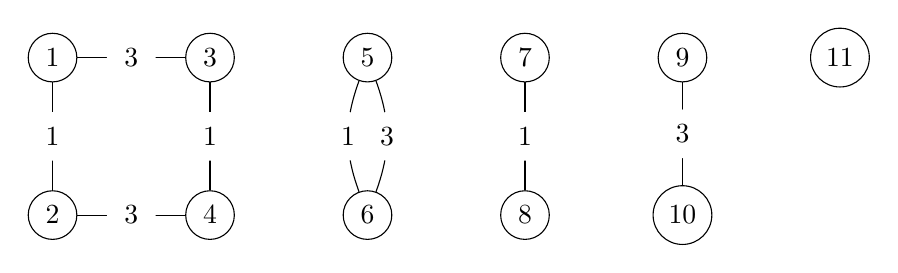
\begin{tikzpicture}

        \begin{scope}[every node/.style={circle,draw}]
          \node (1)  at (0,2)  {1};
          \node (2)  at (0,0)  {2};
          \node (3)  at (2,2)  {3};
          \node (4)  at (2,0)  {4};
          \node (5)  at (4,2)  {5};
          \node (6)  at (4,0)  {6};
          \node (7)  at (6,2)  {7};
          \node (8)  at (6,0)  {8};
          \node (9)  at (8,2)  {9};
          \node (10) at (8,0)  {10};
          \node (11) at (10,2) {11};
        \end{scope}

        \begin{scope}[every node/.style={fill=white,circle}]

          \begin{scope}[every edge/.style={draw}]
            \path (1)  edge node {$1$} (2);
            \path (3)  edge node {$1$} (4);
            \path (5)  edge[bend right=20] node {$1$} (6);
            \path (7)  edge node {$1$} (8);
            \path (1)  edge node {$3$} (3);
            \path (2)  edge node {$3$} (4);
            \path (5)  edge[bend left=20] node {$3$} (6);
            \path (9)  edge node {$3$} (10);
          \end{scope}
        \end{scope}

      \end{tikzpicture}
      \caption{}
    \end{center}
  \end{figure}

  \paragraph{}
  Essayons de placer les involutions $\rho_0$, celles-ci doivent commuter avec $\rho_3$. On peut placer facilement un arête pour relier l'arête simple avec $\rho_1$ au point fixe. Mais pour l'autre c'est plus compliqué. Il faut trouver une arête $\rho_2$ unqiement contenue entre deux arêtes $\rho_1$. A priori, ça parait impossible mais en regardant bien, sur le carré alterne, nous avons deux cotés (les arêtes $\rho_3$) sont placées entre deux arêtes $\rho_1$. Mais ces arêtes ne sont pas $\rho_2$. On peut cependant rajouter une arête $\rho_2$ pour doubler l'arête $\rho_3$ et maintenant on peut la tripler avec $\rho_0$. On a donc

  \begin{figure}[H]
    \begin{center}
      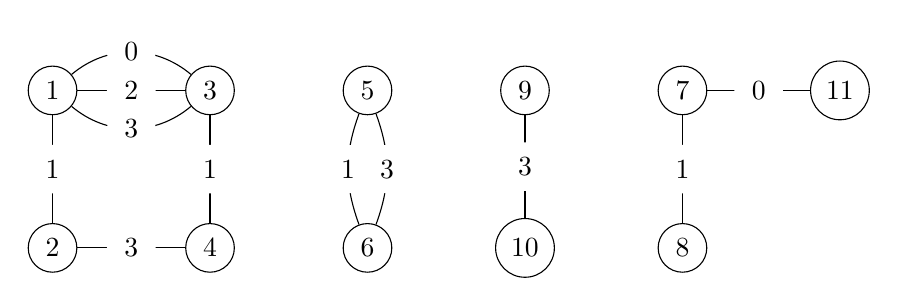
\begin{tikzpicture}

        \begin{scope}[every node/.style={circle,draw}]
          \node (1)  at (0,2)  {1};
          \node (2)  at (0,0)  {2};
          \node (3)  at (2,2)  {3};
          \node (4)  at (2,0)  {4};
          \node (5)  at (4,2)  {5};
          \node (6)  at (4,0)  {6};
          \node (7)  at (8,2)  {7};
          \node (8)  at (8,0)  {8};
          \node (9)  at (6,2)  {9};
          \node (10) at (6,0)  {10};
          \node (11) at (10,2) {11};
        \end{scope}

        \begin{scope}[every node/.style={fill=white,circle}]

          \begin{scope}[every edge/.style={draw}]
            \path (1)  edge[bend left=40] node {$0$} (3);
            \path (7)  edge node {$0$} (11);
            \path (1)  edge node {$1$} (2);
            \path (3)  edge node {$1$} (4);
            \path (5)  edge[bend right=20] node {$1$} (6);
            \path (7)  edge node {$1$} (8);
            \path (1)  edge node {$2$} (3);
            \path (1)  edge[bend right=40] node {$3$} (3);
            \path (2)  edge node {$3$} (4);
            \path (5)  edge[bend left=20] node {$3$} (6);
            \path (9)  edge node {$3$} (10);
          \end{scope}
        \end{scope}

      \end{tikzpicture}
      \caption{}
    \end{center}
  \end{figure}

  \paragraph{}
  Les trois dernières arêtes de $\rho_2$ doivent servir à relier les trois composantes connexes du graphe ci-dessus, sachant que l'arête 0 ne peut être relié à rien et qu'on ne sait créer que deux branches sur le carré alterné. Il y a donc 2 possibilités (une seule branche) plus 2 possibilités (deux branches, la branche avec $\rho_0$ ne contient aucune autre composante) plus 2 possibilités (deux branches, la branche avec $\rho_0$ contient deux composantes). On a donc exactement 6 possibilités.

\end{proof}

\subsection{Quatre 4-transposisitions}

\begin{theorem}
  Tout sggi de rang 4 sur $A_{11}$, composé de quatre 4-transpositions ne peut être un string C-group.
\end{theorem}

\begin{proof}
  Commençons donc par placer les involutions $\rho_1$ et $\rho_3$ qui doivent commuter. Le nombre d'arête libre dans ce cas est de 6. Dans ce cas-ci, nous allons utiliser un autre paramètre. Avec quatre 4-transpositions, nous devons placer 16 arêtes sur le graphe soit 32 extrémités, et nous n'avons que 11 sommets. Ce qui fait que chaque sommet doit avoir, en moyenne $\frac{32}{11} \approx 2,91$, arêtes. Donc, en partant du nombre maximal de $4 \times 11 = 44$, nous ne pouvons perdre que 12 arête par sommet.
  %Les seules structures qui permettent de fixer 4 arêtes par sommet sont les carrés alternés avec une arête triplée présenté pour le cas précédent. Mais ceux-ci ne permettent que d'avoir deux sommets sur lequel il est encore possible d'attacher quelque-chose et cela doit être une arête de $\rho_2$ ou un carré alterné.


  \paragraph{}
  Commençons avec le graphe habituel contenant la 4-transposition $\rho_1$.

  \begin{figure}[H]
    \begin{center}
      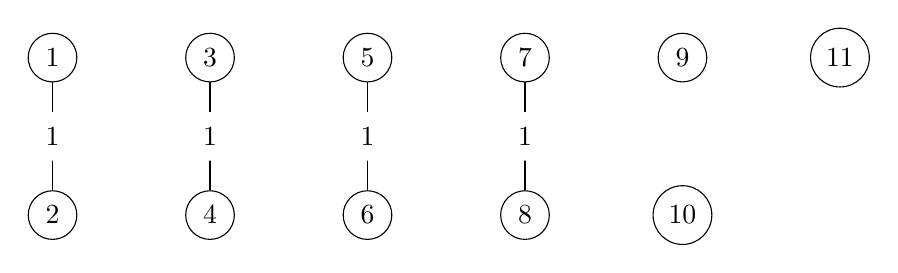
\begin{tikzpicture}

        \begin{scope}[every node/.style={circle,draw}]
          \node (1)  at (0,2)  {1};
          \node (2)  at (0,0)  {2};
          \node (3)  at (2,2)  {3};
          \node (4)  at (2,0)  {4};
          \node (5)  at (4,2)  {5};
          \node (6)  at (4,0)  {6};
          \node (7)  at (6,2)  {7};
          \node (8)  at (6,0)  {8};
          \node (9)  at (8,2)  {9};
          \node (10) at (8,0)  {10};
          \node (11) at (10,2) {11};
        \end{scope}

        \begin{scope}[every node/.style={fill=white,circle}]

          \begin{scope}[every edge/.style={draw}]
            \path (1)  edge node {$1$} (2);
            \path (3)  edge node {$1$} (4);
            \path (5)  edge node {$1$} (6);
            \path (7)  edge node {$1$} (8);
          \end{scope}
        \end{scope}

      \end{tikzpicture}
      \caption{}
    \end{center}
  \end{figure}

  \paragraph{}
  Ensuite, il nous faut rajouter l'involution $\rho_3$, comme d'habitude nous avons le choix entre trois possibilités : un carré alterné, deux doublements ou un doublement et relier deux points fixes. Nous ne pouvons pas utiliser de deux doublements car cela nous bloquerait (TODO). De même pour deux carrés alternés (TODO aussi).

  \paragraph{}
  Nous devons donc utiliser un carré alterné, un doublement et relier deux points fixes. On obtient

  \begin{figure}[H]
    \begin{center}
      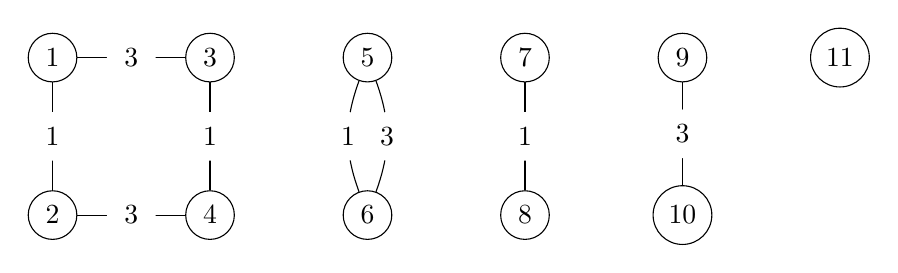
\begin{tikzpicture}

        \begin{scope}[every node/.style={circle,draw}]
          \node (1)  at (0,2)  {1};
          \node (2)  at (0,0)  {2};
          \node (3)  at (2,2)  {3};
          \node (4)  at (2,0)  {4};
          \node (5)  at (4,2)  {5};
          \node (6)  at (4,0)  {6};
          \node (7)  at (6,2)  {7};
          \node (8)  at (6,0)  {8};
          \node (9)  at (8,2)  {9};
          \node (10) at (8,0)  {10};
          \node (11) at (10,2) {11};
        \end{scope}

        \begin{scope}[every node/.style={fill=white,circle}]

          \begin{scope}[every edge/.style={draw}]
            \path (1)  edge node {$1$} (2);
            \path (3)  edge node {$1$} (4);
            \path (5)  edge[bend right=20] node {$1$} (6);
            \path (7)  edge node {$1$} (8);
            \path (1)  edge node {$3$} (3);
            \path (2)  edge node {$3$} (4);
            \path (5)  edge[bend left=20] node {$3$} (6);
            \path (9)  edge node {$3$} (10);
          \end{scope}
        \end{scope}

      \end{tikzpicture}
      \caption{}
    \end{center}
  \end{figure}


  \paragraph{}
  Essayons maitenant de placer l'involution $\rho_0$. Cette involution doit commuter avec $\rho_3$, on a donc les mêmes contraintes que ci-dessus et elle doit former exactement un carré alterné, un doublement d'arête et relier deux points fixés par $\rho_3$. Les deux carrés doivent être adjacents sinon nous n'avons plus de place pour l'involution $\rho_2$. De plus le carré doit utiliser l'arête double précédemment formée et, par symmétrie, l'arête double qu'il forme doit être dans le carré créé à l'étape précédente (TODO). On a donc

  \begin{figure}[H]
    \begin{center}
      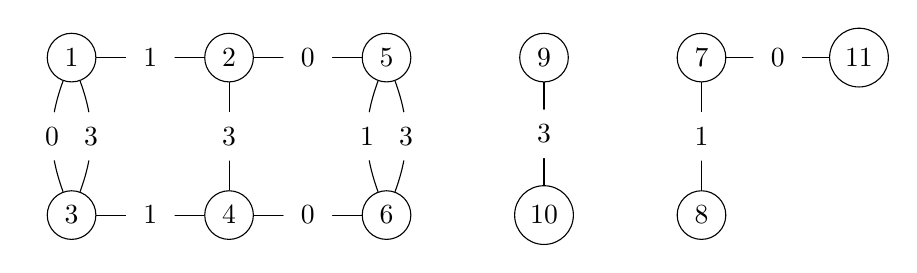
\begin{tikzpicture}

        \begin{scope}[every node/.style={circle,draw}]
          \node (1)  at (0,2)  {1};
          \node (2)  at (2,2)  {2};
          \node (3)  at (0,0)  {3};
          \node (4)  at (2,0)  {4};
          \node (5)  at (4,2)  {5};
          \node (6)  at (4,0)  {6};
          \node (7)  at (8,2)  {7};
          \node (8)  at (8,0)  {8};
          \node (9)  at (6,2)  {9};
          \node (10) at (6,0)  {10};
          \node (11) at (10,2) {11};
        \end{scope}

        \begin{scope}[every node/.style={fill=white,circle}]

          \begin{scope}[every edge/.style={draw}]
            \path (2)  edge node {$0$} (5);
            \path (4)  edge node {$0$} (6);
            \path (1)  edge[bend right=20] node {$0$} (3);
            \path (7)  edge node {$0$} (11);
            \path (1)  edge node {$1$} (2);
            \path (3)  edge node {$1$} (4);
            \path (5)  edge[bend right=20] node {$1$} (6);
            \path (7)  edge node {$1$} (8);
            \path (1)  edge[bend left=20] node {$3$} (3);
            \path (2)  edge node {$3$} (4);
            \path (5)  edge[bend left=20] node {$3$} (6);
            \path (9)  edge node {$3$} (10);
          \end{scope}
        \end{scope}

      \end{tikzpicture}
      \caption{}
    \end{center}
  \end{figure}

  \paragraph{}
  Maintenant il nous faut ajouter l'involution $\rho_2$ qui doit commuter avec $\rho_0$ de telle sorte que ce graphe soit transitif. Commençons par remarquer qu'il est impossible de raccorder directement l'arête $\rho_3$ isolée sur les deux carrés alternés. En effet, vu que nous sommes obligés d'utiliser $\rho_2$, nous ne pouvons pas utiliser les deux points centraux car ils sont connectés à une arête $\rho_0$ et il n'est pas possible de former de carré car nous aurions utilisé nos 4 arêtes et le graphe ne serait pas transitif. De même, nous ne pour l'arête double avec $\rho_0$. Pour l'arête double avec $\rho_1$, ces sommets sont adjacents à des arêtes $\rho_1$ donc c'est aussi impossible.

  \paragraph{}
  Il faut donc raccoder, dans l'ordre, les carrés adjacent aux deux arêtes $\rho_1$ et $\rho_2$ puis raccorder ceci à l'arête $\rho_3$. Dans le premier raccordement, nous devons former un carré alterné avec les arêtes $\rho_2$. Ce qui nous donne le graphe suivant.

  \begin{figure}[H]
    \begin{center}
      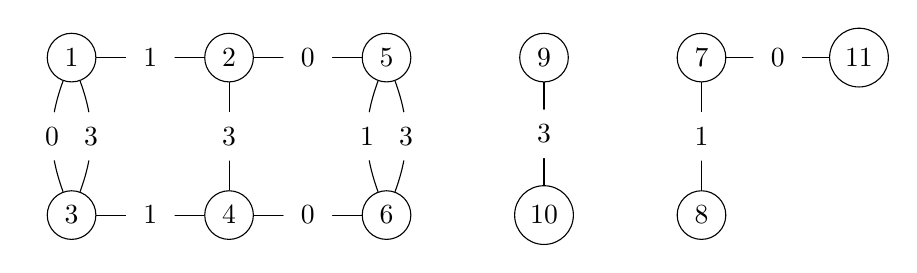
\begin{tikzpicture}

        \begin{scope}[every node/.style={circle,draw}]
          \node (1)  at (0,2)  {1};
          \node (2)  at (2,2)  {2};
          \node (3)  at (0,0)  {3};
          \node (4)  at (2,0)  {4};
          \node (5)  at (4,2)  {5};
          \node (6)  at (4,0)  {6};
          \node (7)  at (8,2)  {7};
          \node (8)  at (8,0)  {8};
          \node (9)  at (6,2)  {9};
          \node (10) at (6,0)  {10};
          \node (11) at (10,2) {11};
        \end{scope}

        \begin{scope}[every node/.style={fill=white,circle}]

          \begin{scope}[every edge/.style={draw}]
            \path (2)  edge node {$0$} (5);
            \path (4)  edge node {$0$} (6);
            \path (1)  edge[bend right=20] node {$0$} (3);
            \path (7)  edge node {$0$} (11);
            \path (1)  edge node {$1$} (2);
            \path (3)  edge node {$1$} (4);
            \path (5)  edge[bend right=20] node {$1$} (6);
            \path (7)  edge node {$1$} (8);
            \path (1)  edge[bend left=20] node {$3$} (3);
            \path (2)  edge node {$3$} (4);
            \path (5)  edge[bend left=20] node {$3$} (6);
            \path (9)  edge node {$3$} (10);
          \end{scope}
        \end{scope}

      \end{tikzpicture}
      \caption{}
    \end{center}
  \end{figure}


\end{proof}
